\documentclass[conference]{IEEEtran}
\IEEEoverridecommandlockouts
% The preceding line is only needed to identify funding in the first footnote. If that is unneeded, please comment it out.
\usepackage{cite}
\usepackage{amsmath,amssymb,amsfonts}
\usepackage{algorithmic}
\usepackage{graphicx}
\usepackage{textcomp}
\usepackage{xcolor}
\def\BibTeX{{\rm B\kern-.05em{\sc i\kern-.025em b}\kern-.08em
    T\kern-.1667em\lower.7ex\hbox{E}\kern-.125emX}}
\begin{document}

\title{Felix Paper Title*\\
{\footnotesize \textsuperscript{*}Note: Sub-titles are not captured in Xplore and
should not be used}
\thanks{Identify applicable funding agency here. If none, delete this.}
}

\author{\IEEEauthorblockN{Felix Girke}
\IEEEauthorblockA{\textit{Computer Science and Engineering} \\
\textit{Frankfurt University of Applied Science}\\
Frankfurt, Germany \\
https://orcid.org/0009-0004-3967-6750}
\and
\IEEEauthorblockN{2\textsuperscript{nd} Given Name Surname}
\IEEEauthorblockA{\textit{dept. name of organization (of Aff.)} \\
\textit{name of organization (of Aff.)}\\
City, Country \\
email address or ORCID}
\and
\IEEEauthorblockN{3\textsuperscript{rd} Given Name Surname}
\IEEEauthorblockA{\textit{dept. name of organization (of Aff.)} \\
\textit{name of organization (of Aff.)}\\
City, Country \\
email address or ORCID}
}

\maketitle

\begin{abstract}
To solve the problem of different interfaces for different robots a data connector is developed.
It creates a interoperable, decentralized Network for a robot system using the Open Platform Communication Unified Architecture (OPC-UA) standard.
Creating a flexible digital twin in Isaac Sim to visualize the data of the robot system.
Remote access to the data connectors (and the digital twin) to monitor the robot system from everywhere.
\end{abstract}

\begin{IEEEkeywords}
OPC-UA, interoperable, decentralized, digital Twin, Isaac Sim, remote access
\end{IEEEkeywords}

\section{Introduction}
Every robot manufacturer develops uses their own way of communication with their robot.
This leads to problems when trying to build a robot system with multiple robots from different brands.
In this example two robot arms from Kinova are to be mounted on a Husky mobile robot platform from Clearpath.
The Husky uses Robot Operating System (ROS) to communicate internally while the robot arms use the Kortex api from Kinova.
To combine them into one digital twin they should be on one standard.
For this a data connector is developed on the Open Platform Communication Unified Architecture (OPC-UA) standard.
Its purpose is to act as a layer between the robot specific language and the outside world, in this example the digital twin.
To add flexibility the robot data isn't collected on one server but every robot has its own server.
Because of this decentralized approach every client can choose to connect only to the servers it wants to.
For example if only one of the robot arms is mounted on the husky the digital twin can connect to only this one while the other robot arm con be used otherwise.
\section{Advantages of OPC-UA}
was ist opcua? \cite{OPCUA}
warum opcua
sprich semantische Interoperabilität, Ressourcenschonung (Subscribe und Publish statt Polling), …das wäre Kap. 3.1

\section{Development of the data connector}
Depending on the robot it might be possible to install software onto it.
If this is the case there is no need for additional Hardware .
On the Husky PC runs ROS, so it is possible to create an ROS package with a OPC-UA Server.
On the Kinova robot arms on the other Hand it is not possible to install software, so an Raspberry Pi is used which gets the data from the robot and makes them accessible via an OPC-UA server.
To simplify the development the OPC-UA Server code is implemented as a stand-alone class, so it can be reused for different robots.
\subsection{As a ROS package}
\subsection{As a stand-alone device}
As Hardware for the stand-alone device a Raspberry PI 3B+ is used because it is very versatile. It could connect to robots via Ethernet, USB or with the GPIO pin nearly every other connection standard.
Furthermore it is powerful enough to handle an OPC-UA server and talk to an robot at the same time.
The Code is split into three main parts (Fig. \ref{fig:dataConectorStructure}).
\begin{figure}[htbp]
    \centerline{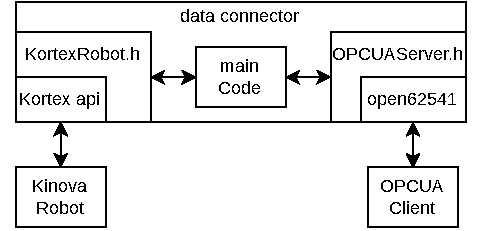
\includegraphics{Pictures/dataConectorStructure.pdf}}
    \caption{Code structure of the data connector}
    \label{fig:dataConectorStructure}
\end{figure}
One part is the communication to the robot via the Kortex api, the second part is the OPC-UA server with the open62541 library.
The main code part in the middle  starts a thread for the connection to the robot and a thread for the OPC-UA Server.
It also connects the data from from the robot class to the OPC-UA Server class.
So if the connector is used with another robot, it is enough to just write a new connection to the robot.
It is also possible to prepare the connection to a robot from a different manufacturer and let the main code detect what robot is connected.
This increases the flexibility of the data connector. 
% ToDo:
% syncronisation
% rapsi nicht auf der Oberflache bleiben
% batterie soc
% digialen zwilling vor dem kauf durch den Server simulation
\section{Performance Tests}
To ensure the data doesn't take to long from the robot to a client a series of performance tests are conducted.
These can be separate in two parts. 
First getting the data from the robot to the data connector and second get the data from the data connector to the client.
Every test is made with 5 samples. Every sample is the average speed of the first 1000 data requests.
\subsection{Getting data from the robot}
The Raspberry Pi 3B+ is directly connected to the Kinova robot via a ethernet cable.
With UDP as communication standard the Raspberry Pi can get the up to 1400 datasets per second from the Kinova robot (Fig. \ref{fig:KortexAPISpeed}).
That is even more than the 1000 datasets per second, that Kinova claims \cite{KortexUDP}.
\begin{figure}[htbp]
    \centerline{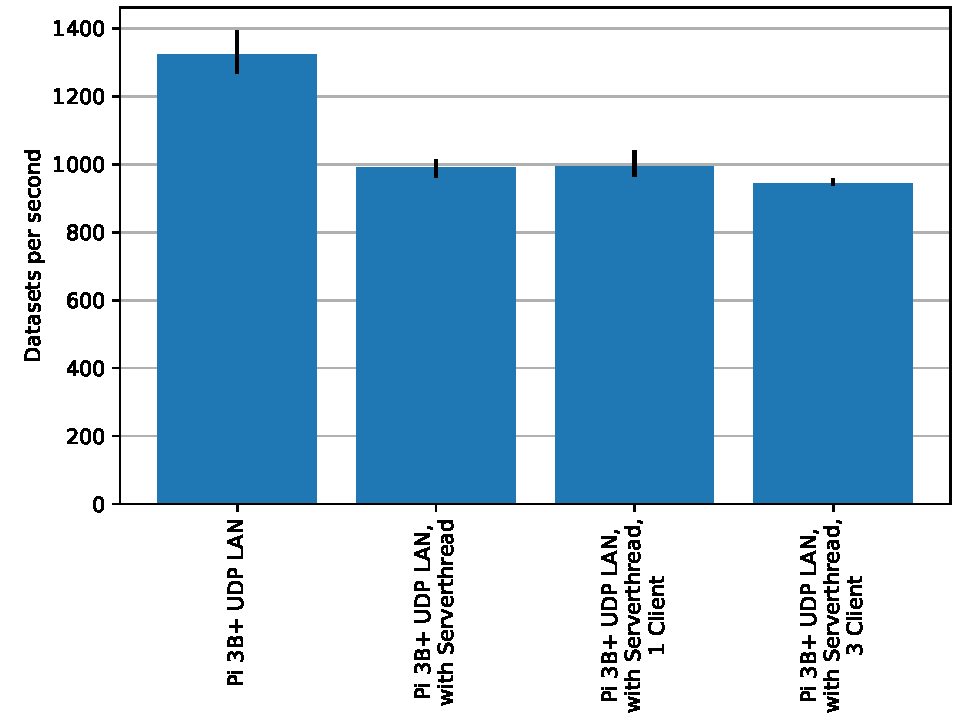
\includegraphics[width=8cm]{Pictures/KortexAPISpeed.pdf}}
    \caption{Frequency with which the Raspberry Pi 3B+ can get data from the Kinova arm}
    \label{fig:KortexAPISpeed}
\end{figure}
A dataset consists of all the data the robot has to offer. Thats over 50 data points.
Is the OPC-UA server is running parallel on the Raspberry Pi the frequency is lower, around 1kHz.
If one client is simultaneously requesting data from the OPC-UA server the frequency isn't really affected.
But if there are more clients then the frequency begins to drop slowly.
\subsection{Getting Data from the data connector}
To get the data from the data connector two different PCs are used. One midrange Laptop (Intel 11.Gen Core i7-1165G7, Realtek Semiconductor
RTL8152 Fast Ethernet Adapter) and an high end Tower PC (Intel 13.Gen Core i9-13900KF, Realtek Gaming R2.5GbE Family Controller).
The PCs and the data connector are all connected to a Router (tp-link Archer C80 AC1900 MU-MiMO).\\
\begin{figure}[htbp]
    \centerline{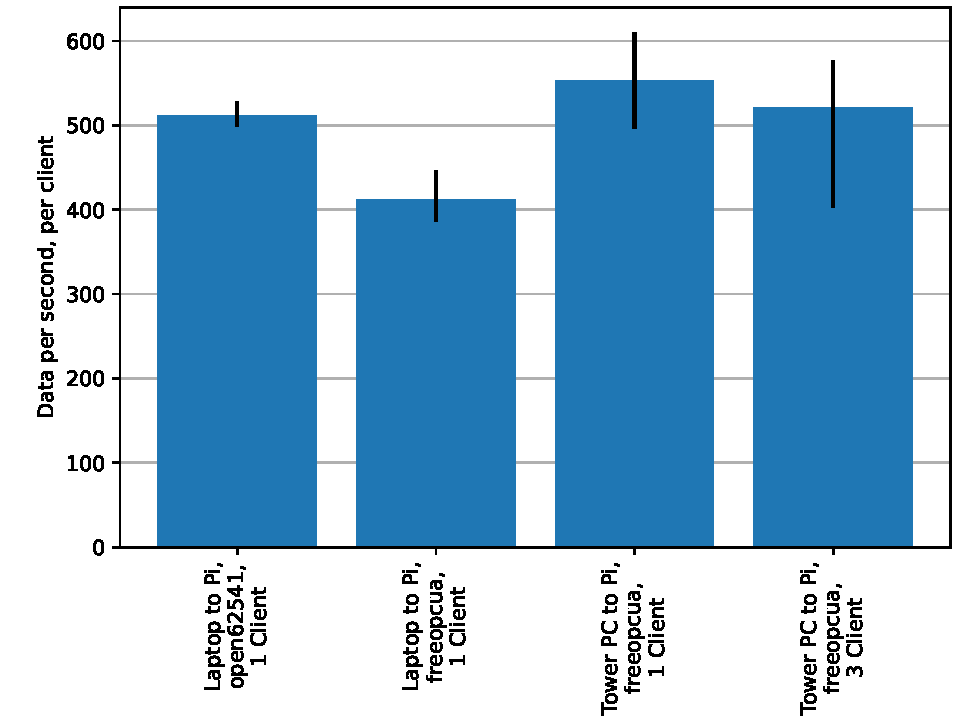
\includegraphics[width=8cm]{Pictures/OPCUASpeed1D.pdf}}
    \caption{Frequency with which data can be requested from the OPC-UA server}
    \label{fig:OPCUASpeed1D}
\end{figure}
In Fig. \ref{fig:OPCUASpeed1D} different libraries are used for the client to request one Value from the data connector.
On the Laptop the c-library open62541 is faster than the python library freeopcua.
On the Tower PC the python library is even faster than the c library on the Laptop.
If these results are compared to the ping between these PCs and the data connector (Fig. \ref{fig:PingDiagram}) it can be concluded that the python library on the Tower PC is running close to the actual limit of the network.\\
\begin{figure}[htbp]
    \centerline{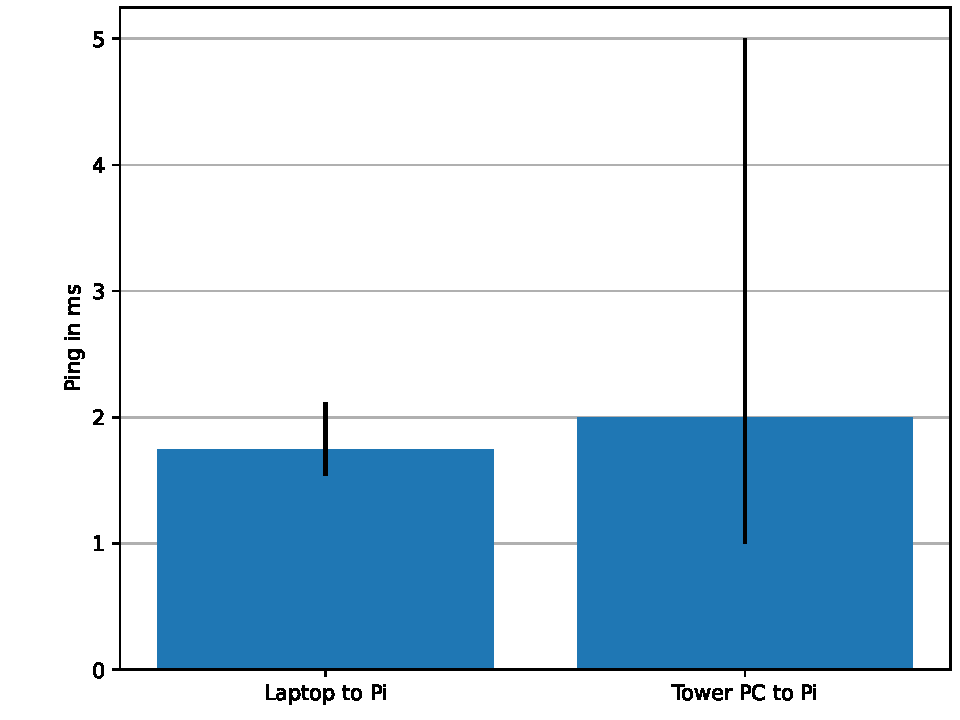
\includegraphics[width=8cm]{Pictures/PingDiagram.pdf}}
    \caption{Ping to the data connector}
    \label{fig:PingDiagram}
\end{figure}
If multiple clients are started in parallel on the Tower PC there is a slight decrease in the frequency with which the data can be requested from the data connector (Fig. \ref{fig:OPCUASpeed1D}).
\begin{figure}[htbp]
    \centerline{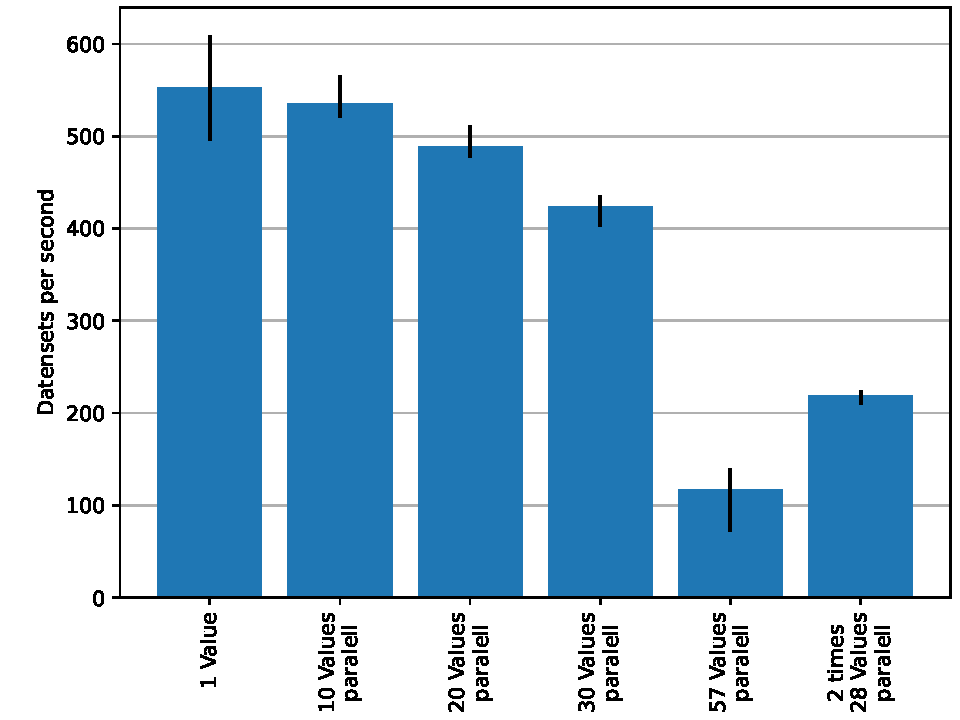
\includegraphics[width=8cm]{Pictures/OPCUAMultipleDatenAufEinmal.pdf}}
    \caption{Frequency with which different datasets can be requested from the OPC-UA server}
    \label{fig:OPCUAMultipleDatenAufEinmal}
\end{figure}
In the last test (Fig. \ref{fig:OPCUAMultipleDatenAufEinmal}) datasets with different amounts of values are requested from the data connector via the Tower PC using the python library.

\section{Digital twin}
\section{Remote access}
\newpage
\newpage
\section{Ease of Use}

\subsection{Maintaining the Integrity of the Specifications}

The IEEEtran class file is used to format your paper and style the text. All margins, 
column widths, line spaces, and text fonts are prescribed; please do not 
alter them. You may note peculiarities. For example, the head margin
measures proportionately more than is customary. This measurement 
and others are deliberate, using specifications that anticipate your paper 
as one part of the entire proceedings, and not as an independent document. 
Please do not revise any of the current designations.

\section{Prepare Your Paper Before Styling}
Before you begin to format your paper, first write and save the content as a 
separate text file. Complete all content and organizational editing before 
formatting. Please note sections \ref{AA}--\ref{SCM} below for more information on 
proofreading, spelling and grammar.

Keep your text and graphic files separate until after the text has been 
formatted and styled. Do not number text heads---{\LaTeX} will do that 
for you.

\subsection{Abbreviations and Acronyms}\label{AA}
Define abbreviations and acronyms the first time they are used in the text, 
even after they have been defined in the abstract. Abbreviations such as 
IEEE, SI, MKS, CGS, ac, dc, and rms do not have to be defined. Do not use 
abbreviations in the title or heads unless they are unavoidable.

\subsection{Units}
\begin{itemize}
\item Use either SI (MKS) or CGS as primary units. (SI units are encouraged.) English units may be used as secondary units (in parentheses). An exception would be the use of English units as identifiers in trade, such as ``3.5-inch disk drive''.
\item Avoid combining SI and CGS units, such as current in amperes and magnetic field in oersteds. This often leads to confusion because equations do not balance dimensionally. If you must use mixed units, clearly state the units for each quantity that you use in an equation.
\item Do not mix complete spellings and abbreviations of units: ``Wb/m\textsuperscript{2}'' or ``webers per square meter'', not ``webers/m\textsuperscript{2}''. Spell out units when they appear in text: ``. . . a few henries'', not ``. . . a few H''.
\item Use a zero before decimal points: ``0.25'', not ``.25''. Use ``cm\textsuperscript{3}'', not ``cc''.)
\end{itemize}

\subsection{Equations}
Number equations consecutively. To make your 
equations more compact, you may use the solidus (~/~), the exp function, or 
appropriate exponents. Italicize Roman symbols for quantities and variables, 
but not Greek symbols. Use a long dash rather than a hyphen for a minus 
sign. Punctuate equations with commas or periods when they are part of a 
sentence, as in:
\begin{equation}
a+b=\gamma\label{eq}
\end{equation}

Be sure that the 
symbols in your equation have been defined before or immediately following 
the equation. Use ``\eqref{eq}'', not ``Eq.~\eqref{eq}'' or ``equation \eqref{eq}'', except at 
the beginning of a sentence: ``Equation \eqref{eq} is . . .''

\subsection{\LaTeX-Specific Advice}

Please use ``soft'' (e.g., \verb|\eqref{Eq}|) cross references instead
of ``hard'' references (e.g., \verb|(1)|). That will make it possible
to combine sections, add equations, or change the order of figures or
citations without having to go through the file line by line.

Please don't use the \verb|{eqnarray}| equation environment. Use
\verb|{align}| or \verb|{IEEEeqnarray}| instead. The \verb|{eqnarray}|
environment leaves unsightly spaces around relation symbols.

Please note that the \verb|{subequations}| environment in {\LaTeX}
will increment the main equation counter even when there are no
equation numbers displayed. If you forget that, you might write an
article in which the equation numbers skip from (17) to (20), causing
the copy editors to wonder if you've discovered a new method of
counting.

{\BibTeX} does not work by magic. It doesn't get the bibliographic
data from thin air but from .bib files. If you use {\BibTeX} to produce a
bibliography you must send the .bib files. 

{\LaTeX} can't read your mind. If you assign the same label to a
subsubsection and a table, you might find that Table I has been cross
referenced as Table IV-B3. 

{\LaTeX} does not have precognitive abilities. If you put a
\verb|\label| command before the command that updates the counter it's
supposed to be using, the label will pick up the last counter to be
cross referenced instead. In particular, a \verb|\label| command
should not go before the caption of a figure or a table.

Do not use \verb|\nonumber| inside the \verb|{array}| environment. It
will not stop equation numbers inside \verb|{array}| (there won't be
any anyway) and it might stop a wanted equation number in the
surrounding equation.

\subsection{Some Common Mistakes}\label{SCM}
\begin{itemize}
\item The word ``data'' is plural, not singular.
\item The subscript for the permeability of vacuum $\mu_{0}$, and other common scientific constants, is zero with subscript formatting, not a lowercase letter ``o''.
\item In American English, commas, semicolons, periods, question and exclamation marks are located within quotation marks only when a complete thought or name is cited, such as a title or full quotation. When quotation marks are used, instead of a bold or italic typeface, to highlight a word or phrase, punctuation should appear outside of the quotation marks. A parenthetical phrase or statement at the end of a sentence is punctuated outside of the closing parenthesis (like this). (A parenthetical sentence is punctuated within the parentheses.)
\item A graph within a graph is an ``inset'', not an ``insert''. The word alternatively is preferred to the word ``alternately'' (unless you really mean something that alternates).
\item Do not use the word ``essentially'' to mean ``approximately'' or ``effectively''.
\item In your paper title, if the words ``that uses'' can accurately replace the word ``using'', capitalize the ``u''; if not, keep using lower-cased.
\item Be aware of the different meanings of the homophones ``affect'' and ``effect'', ``complement'' and ``compliment'', ``discreet'' and ``discrete'', ``principal'' and ``principle''.
\item Do not confuse ``imply'' and ``infer''.
\item The prefix ``non'' is not a word; it should be joined to the word it modifies, usually without a hyphen.
\item There is no period after the ``et'' in the Latin abbreviation ``et al.''.
\item The abbreviation ``i.e.'' means ``that is'', and the abbreviation ``e.g.'' means ``for example''.
\end{itemize}
An excellent style manual for science writers is \cite{b7}.

\subsection{Authors and Affiliations}
\textbf{The class file is designed for, but not limited to, six authors.} A 
minimum of one author is required for all conference articles. Author names 
should be listed starting from left to right and then moving down to the 
next line. This is the author sequence that will be used in future citations 
and by indexing services. Names should not be listed in columns nor group by 
affiliation. Please keep your affiliations as succinct as possible (for 
example, do not differentiate among departments of the same organization).

\subsection{Identify the Headings}
Headings, or heads, are organizational devices that guide the reader through 
your paper. There are two types: component heads and text heads.

Component heads identify the different components of your paper and are not 
topically subordinate to each other. Examples include Acknowledgments and 
References and, for these, the correct style to use is ``Heading 5''. Use 
``figure caption'' for your Figure captions, and ``table head'' for your 
table title. Run-in heads, such as ``Abstract'', will require you to apply a 
style (in this case, italic) in addition to the style provided by the drop 
down menu to differentiate the head from the text.

Text heads organize the topics on a relational, hierarchical basis. For 
example, the paper title is the primary text head because all subsequent 
material relates and elaborates on this one topic. If there are two or more 
sub-topics, the next level head (uppercase Roman numerals) should be used 
and, conversely, if there are not at least two sub-topics, then no subheads 
should be introduced.

\subsection{Figures and Tables}
\paragraph{Positioning Figures and Tables} Place figures and tables at the top and 
bottom of columns. Avoid placing them in the middle of columns. Large 
figures and tables may span across both columns. Figure captions should be 
below the figures; table heads should appear above the tables. Insert 
figures and tables after they are cited in the text. Use the abbreviation 
``Fig.~\ref{fig}'', even at the beginning of a sentence.

\begin{table}[htbp]
\caption{Table Type Styles}
\begin{center}
\begin{tabular}{|c|c|c|c|}
\hline
\textbf{Table}&\multicolumn{3}{|c|}{\textbf{Table Column Head}} \\
\cline{2-4} 
\textbf{Head} & \textbf{\textit{Table column subhead}}& \textbf{\textit{Subhead}}& \textbf{\textit{Subhead}} \\
\hline
copy& More table copy$^{\mathrm{a}}$& &  \\
\hline
\multicolumn{4}{l}{$^{\mathrm{a}}$Sample of a Table footnote.}
\end{tabular}
\label{tab1}
\end{center}
\end{table}

\begin{figure}[htbp]
\centerline{
\includegraphics{Pictures/fig1.png}}
\caption{Example of a figure caption.}
\label{fig}
\end{figure}

Figure Labels: Use 8 point Times New Roman for Figure labels. Use words 
rather than symbols or abbreviations when writing Figure axis labels to 
avoid confusing the reader. As an example, write the quantity 
``Magnetization'', or ``Magnetization, M'', not just ``M''. If including 
units in the label, present them within parentheses. Do not label axes only 
with units. In the example, write ``Magnetization (A/m)'' or ``Magnetization 
\{A[m(1)]\}'', not just ``A/m''. Do not label axes with a ratio of 
quantities and units. For example, write ``Temperature (K)'', not 
``Temperature/K''.

\section*{Acknowledgment}

The preferred spelling of the word ``acknowledgment'' in America is without 
an ``e'' after the ``g''. Avoid the stilted expression ``one of us (R. B. 
G.) thanks $\ldots$''. Instead, try ``R. B. G. thanks$\ldots$''. Put sponsor 
acknowledgments in the unnumbered footnote on the first page.

\section*{References}

Please number citations consecutively within brackets \cite{b1}. The 
sentence punctuation follows the bracket \cite{b2}. Refer simply to the reference 
number, as in \cite{b3}---do not use ``Ref. \cite{b3}'' or ``reference \cite{b3}'' except at 
the beginning of a sentence: ``Reference \cite{b3} was the first $\ldots$''

Number footnotes separately in superscripts. Place the actual footnote at 
the bottom of the column in which it was cited. Do not put footnotes in the 
abstract or reference list. Use letters for table footnotes.

Unless there are six authors or more give all authors' names; do not use 
``et al.''. Papers that have not been published, even if they have been 
submitted for publication, should be cited as ``unpublished'' \cite{b4}. Papers 
that have been accepted for publication should be cited as ``in press'' \cite{b5}. 
Capitalize only the first word in a paper title, except for proper nouns and 
element symbols.

For papers published in translation journals, please give the English 
citation first, followed by the original foreign-language citation \cite{b6}.

\begin{thebibliography}{00}
\bibitem{OPCUA}https://opcfoundation.org/about/opc-technologies/opc-ua/
\bibitem{KortexUDP} Kinova, Kortex TransportClient classes, https://docs.kinovarobotics.com/kortex/linked\_md/cpp\_transport\_router\_session\_notif.html\#transportclient-classes, last checked 08.02.2024
\bibitem{b1} G. Eason, B. Noble, and I. N. Sneddon, ``On certain integrals of Lipschitz-Hankel type involving products of Bessel functions,'' Phil. Trans. Roy. Soc. London, vol. A247, pp. 529--551, April 1955.
\bibitem{b2} J. Clerk Maxwell, A Treatise on Electricity and Magnetism, 3rd ed., vol. 2. Oxford: Clarendon, 1892, pp.68--73.
\bibitem{b3} I. S. Jacobs and C. P. Bean, ``Fine particles, thin films and exchange anisotropy,'' in Magnetism, vol. III, G. T. Rado and H. Suhl, Eds. New York: Academic, 1963, pp. 271--350.
\bibitem{b4} K. Elissa, ``Title of paper if known,'' unpublished.
\bibitem{b5} R. Nicole, ``Title of paper with only first word capitalized,'' J. Name Stand. Abbrev., in press.
\bibitem{b6} Y. Yorozu, M. Hirano, K. Oka, and Y. Tagawa, ``Electron spectroscopy studies on magneto-optical media and plastic substrate interface,'' IEEE Transl. J. Magn. Japan, vol. 2, pp. 740--741, August 1987 [Digests 9th Annual Conf. Magnetics Japan, p. 301, 1982].
\bibitem{b7} M. Young, The Technical Writer's Handbook. Mill Valley, CA: University Science, 1989.
\end{thebibliography}
\vspace{12pt}
\color{red}
IEEE conference templates contain guidance text for composing and formatting conference papers. Please ensure that all template text is removed from your conference paper prior to submission to the conference. Failure to remove the template text from your paper may result in your paper not being published.

\end{document}
